\chapter{Results}\label{chap:results_rankings}

\begin{figure}[h!]
    \centering
    \begin{subfigure}[b]{0.3\textwidth}
         \centering
          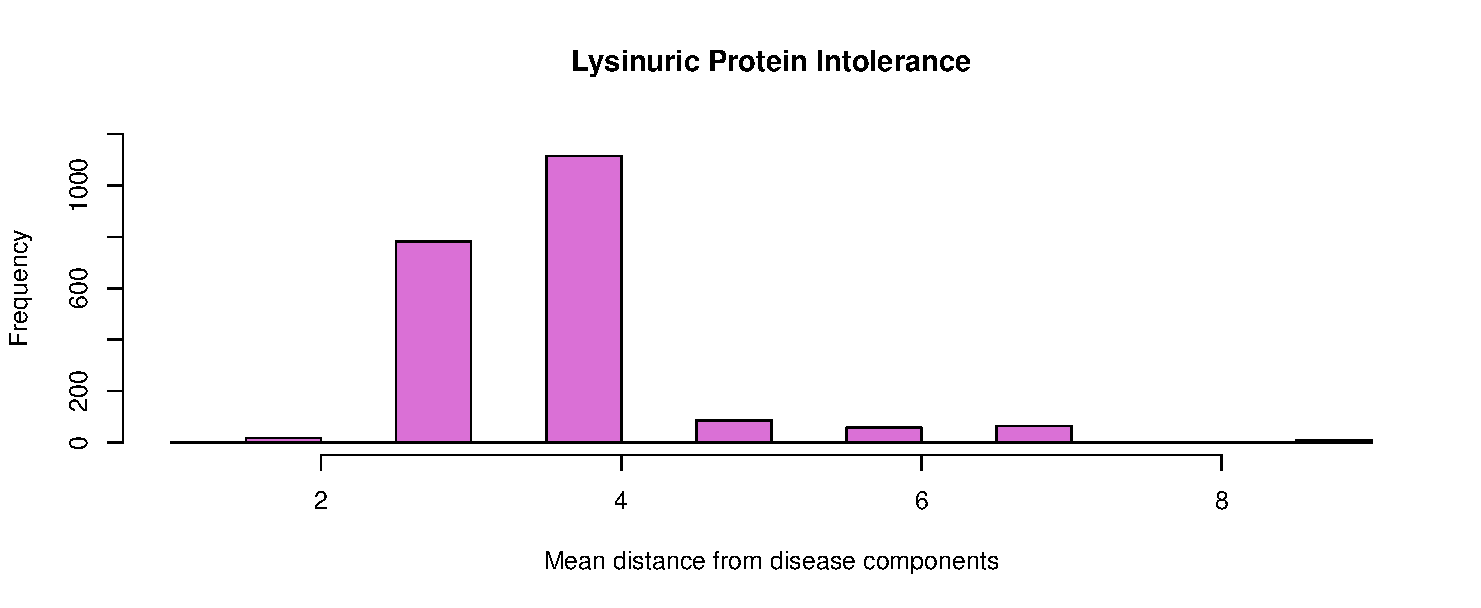
\includegraphics[scale=0.25]{Images/Lisinuric Protein Intolerance.pdf}
         \caption{LPI}
         \label{fig:Lisinuric}
     \end{subfigure}
     \hfill
     \begin{subfigure}[b]{0.3\textwidth}
         \centering
         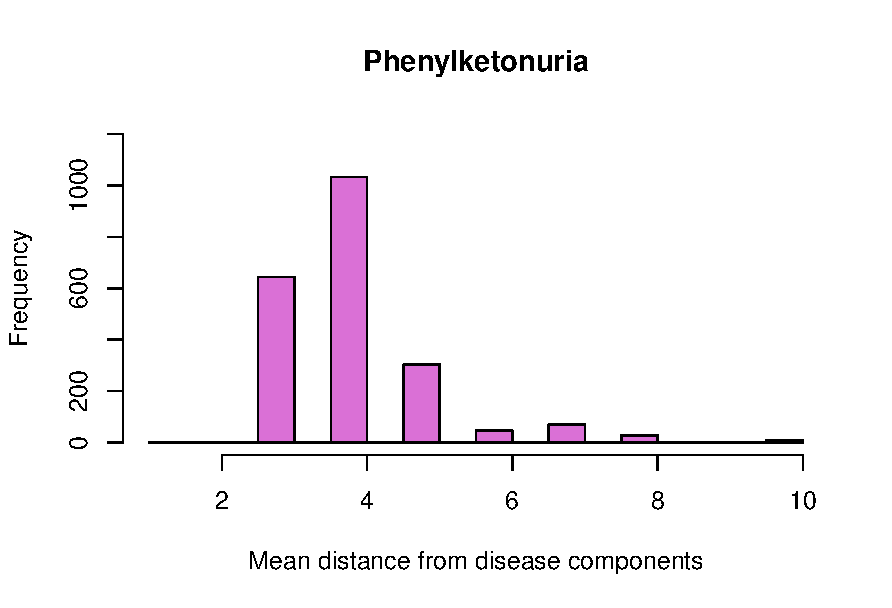
\includegraphics[scale=0.25]{Images/Phenylketonuria.pdf}
         \caption{Phenylketonuria}
         \label{fig:Phenylketonuria}
     \end{subfigure}
     \hfill
     \begin{subfigure}[b]{0.3\textwidth}
         \centering
         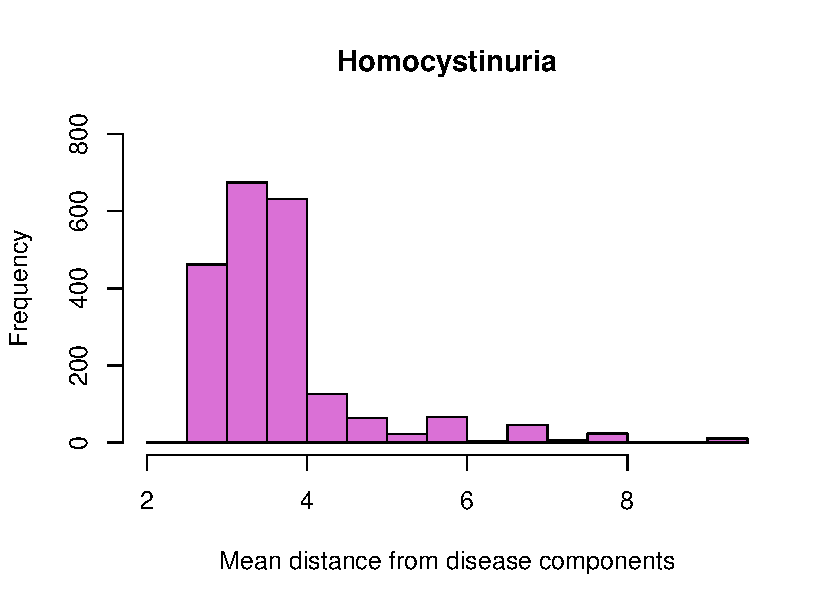
\includegraphics[scale=0.25]{Images/Homocystinuria.pdf}
         \caption{Homocystinuria}
         \label{fig:Homocystinuria}
     \end{subfigure}
     \hfill
     \begin{subfigure}[b]{0.3\textwidth}
         \centering
         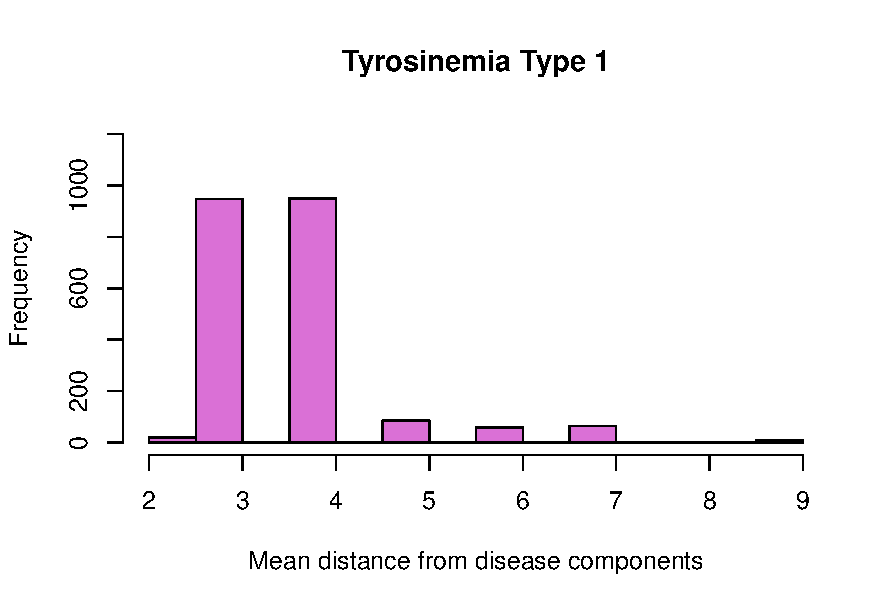
\includegraphics[scale=0.25]{Images/Tyrosinemia Type I.pdf}
         \caption{Tyrosinemia Type I}
         \label{fig:Tyrosinemia Type I}
     \end{subfigure}
     \hfill
     \begin{subfigure}[b]{0.3\textwidth}
         \centering
         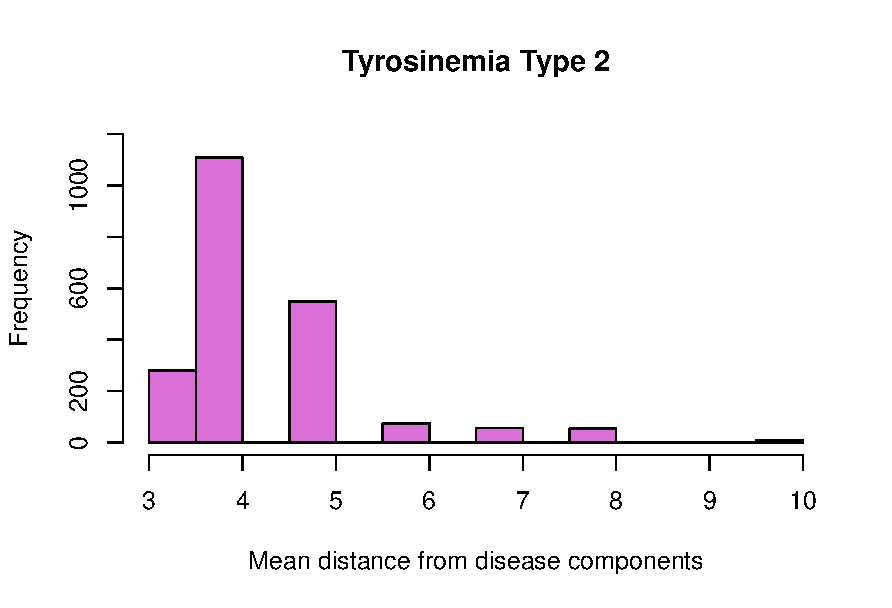
\includegraphics[scale=0.25]{Images/Tyrosinemia Type II.pdf}
         \caption{Tyrosinemia Type II}
         \label{fig:Tyrosinemia Type II}
     \end{subfigure}
     \hfill
     \begin{subfigure}[b]{0.3\textwidth}
         \centering
         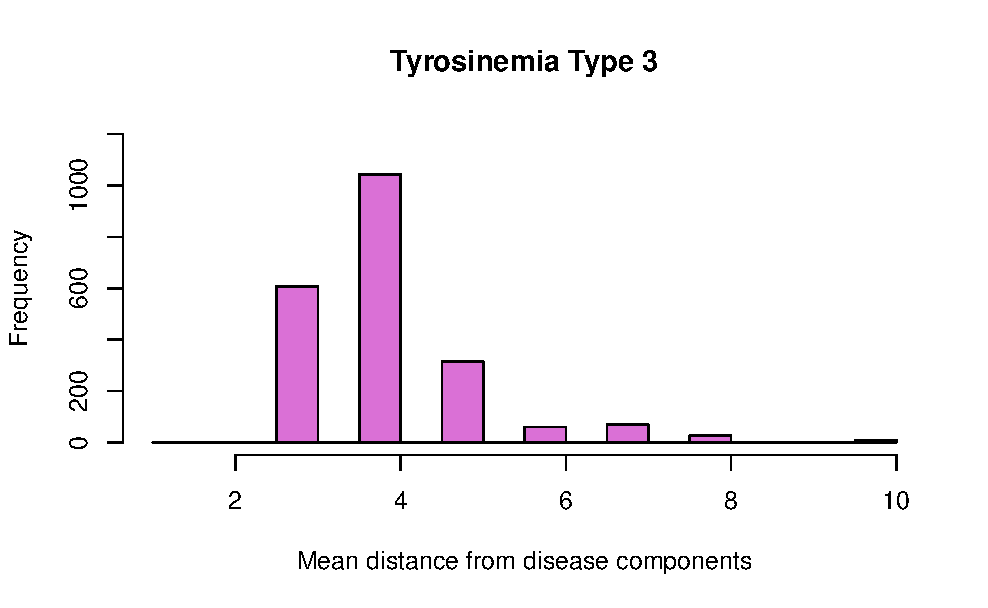
\includegraphics[scale=0.25]{Images/Tyrosinemia Type III.pdf}
         \caption{Tyrosinemia Type III}
         \label{fig:Tyrosinemia Type III}
     \end{subfigure}
     \hfill
     \begin{subfigure}[b]{0.3\textwidth}
         \centering
         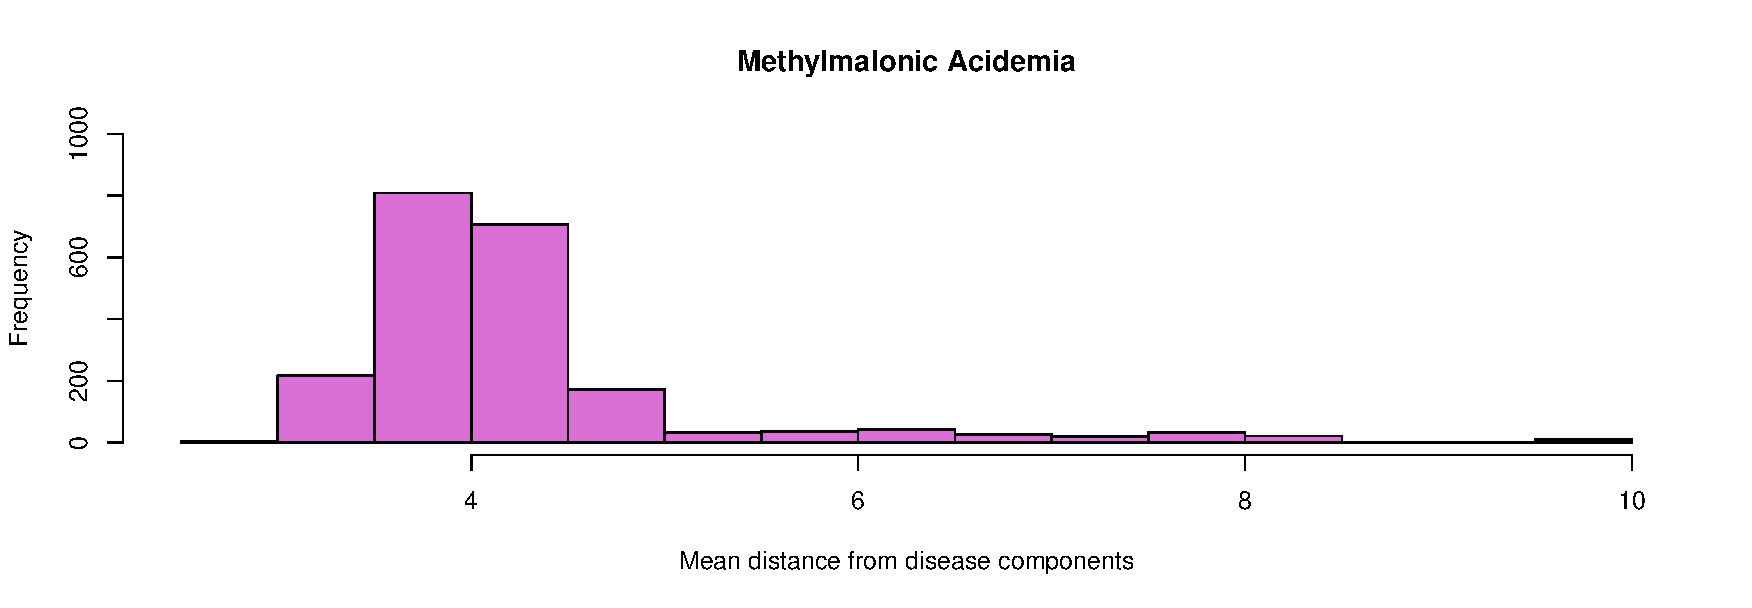
\includegraphics[scale=0.25]{Images/Methylmalonic Acidemia.pdf}
         \caption{Methylmalonic A.}
         \label{fig:Methylmalonic Acidemia}
     \end{subfigure}
     \hfill
     \begin{subfigure}[b]{0.3\textwidth}
         \centering
         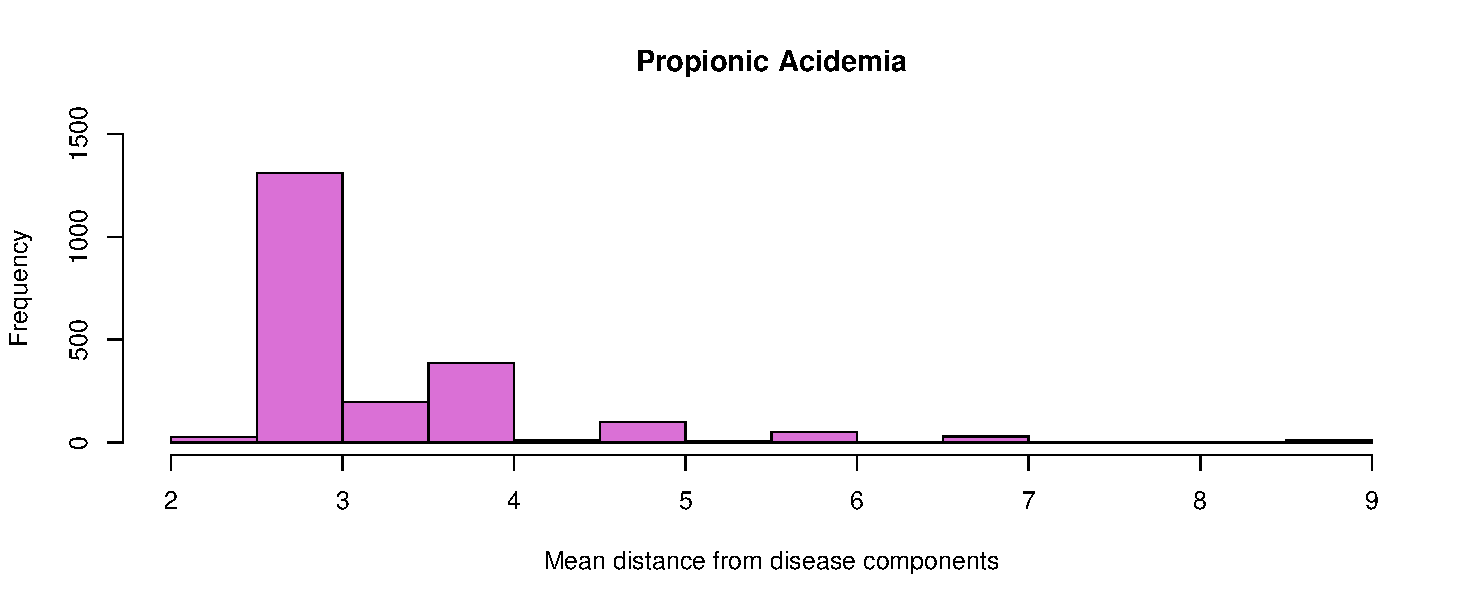
\includegraphics[scale=0.25]{Images/Propionic Acidemia.pdf}
         \caption{Propionic Acidemia}
         \label{fig:Propionic Acidemia}
     \end{subfigure}
     \hfill
     \begin{subfigure}[b]{0.3\textwidth}
         \centering
         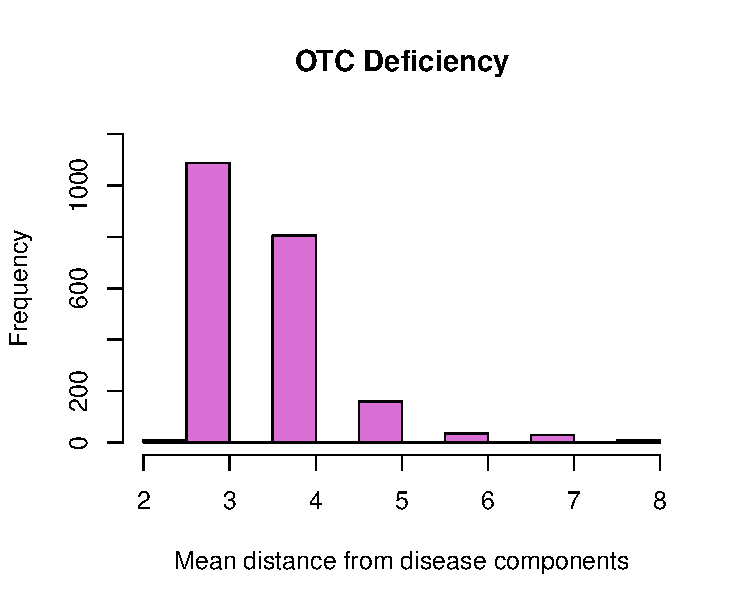
\includegraphics[scale=0.25]{Images/OTC Deficiency.pdf}
         \caption{OTC Deficiency}
         \label{fig:OTC}
     \end{subfigure}
     \hfill
      \begin{subfigure}[b]{0.3\textwidth}
         \centering
         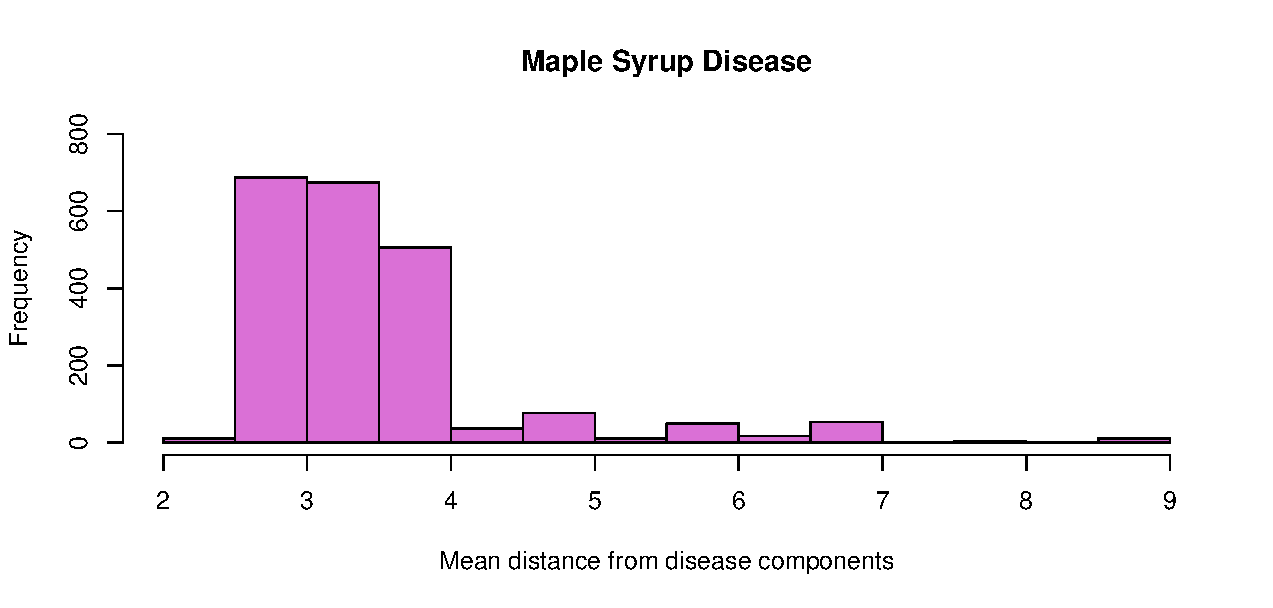
\includegraphics[scale=0.25]{Images/Maple Syrup Disease.pdf}
         \caption{Maple Syrup Disease}
         \label{fig:Maple Syrup}
     \end{subfigure}
     \hfill
     \begin{subfigure}[b]{0.3\textwidth}
         \centering
         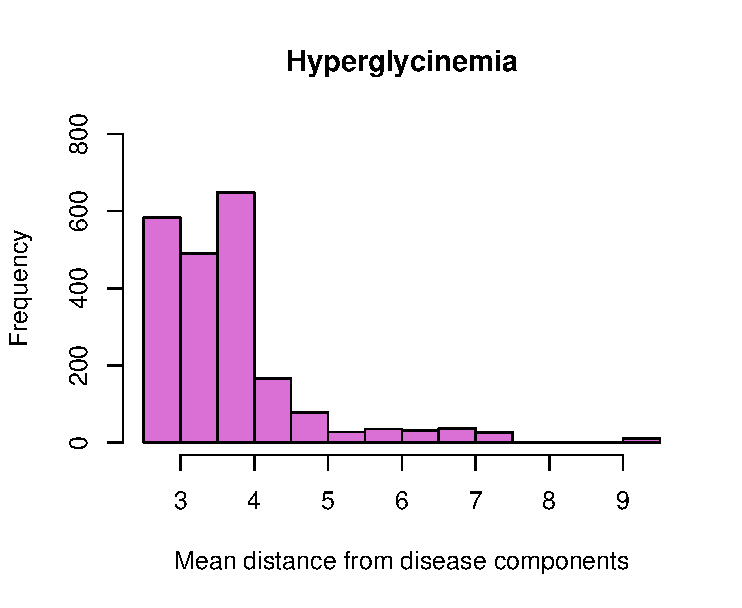
\includegraphics[scale=0.25]{Images/Hyperglycinemia.pdf}
         \caption{Hyperglycinemia}
         \label{fig:Hyperglycinemia}
     \end{subfigure}
     \hfill
     \begin{subfigure}[b]{0.3\textwidth}
         \centering
         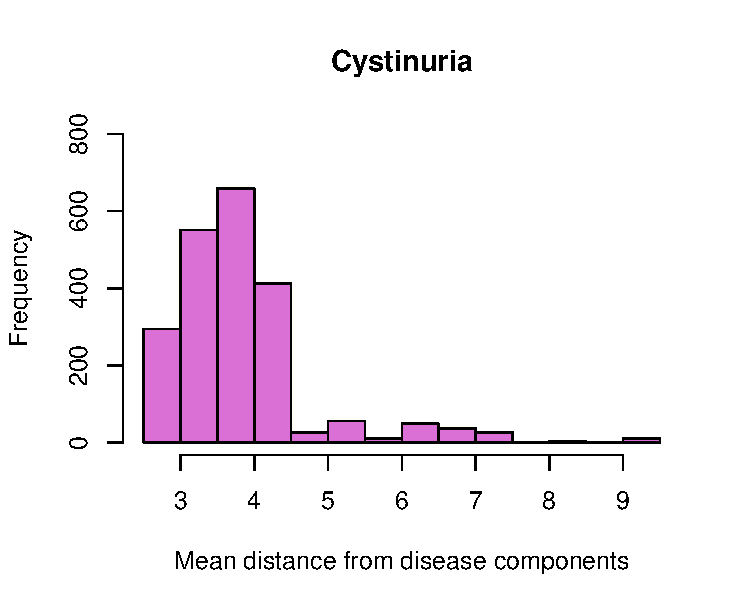
\includegraphics[scale=0.25]{Images/Cystinuria.pdf}
         \caption{Cystinuria}
         \label{fig:Cystinuria}
     \end{subfigure}
     \hfill
    \caption{Drugs mean distances distribution percentages for each disease's ranking}
    \label{fig:results}
\end{figure}
\FloatBarrier